% SemEval-2019 Task 6 paper template for RyanOng
% Based on naacl2019.tex

\documentclass[11pt,a4paper]{article}
\usepackage[hyperref]{naaclhlt2019}
\usepackage{times}
\usepackage{latexsym}
\usepackage{graphicx}
\usepackage{url}

%\aclfinalcopy % Uncomment this line for the final submission
%\def\aclpaperid{***} %  Enter the acl Paper ID here

%\setlength\titlebox{5cm}
% You can expand the titlebox if you need extra space
% to show all the authors. Please do not make the titlebox
% smaller than 5cm (the original size); we will check this
% in the camera-ready version and ask you to change it back.

\newcommand\BibTeX{B{\sc ib}\TeX}

% You can change the part that says "Your Paper Title"
\title{RyanOng at SemEval-2019 Task 6: Your Paper Title}
% NOTE:
% Give your paper a descriptive title, possibly mentioning your methodology/approach.

\author{First Author \\
  Affiliation / Address line 1 \\
  Affiliation / Address line 2 \\
  Affiliation / Address line 3 \\
  {\tt email@domain} \\\And
  Second Author \\
  Affiliation / Address line 1 \\
  Affiliation / Address line 2 \\
  Affiliation / Address line 3 \\
  {\tt email@domain} \\}

\date{}

\begin{document}
\maketitle
\begin{abstract}
This document contains the instructions for preparing a camera-ready manuscript for the proceedings of SemEval 2019.
%
The document itself conforms to its own specifications, and is therefore an example of what your manuscript should look like.
%
\bf Please write a brief \emph{abstract} describing your system and the results you obtained. You can also briefly mention any insights or interesting highlights from your results. We recommend you to include the name of your team in the abstract.
\end{abstract}

\section*{Practical Information}

This paper represents an example of how a system description paper may be structured. We included tables and confusion matrices with the results of your submissions to speed up writing. A bib file with relevant references is also included.
\\

{\bf Paper Title:} SemEval has its own paper naming conventions. The title of your paper should be according to the title of this template, that is:\\

{\bf TEAM NAME at SemEval-2019 Task 6: Paper Title} 
\\

{\bf Team Name:} {\bf IMPORTANT} Your team name should be the {\bf same} as the name you used at CodaLab.  This is the name that appear in the ranks and in the shared task report. If you choose to change your team name now, readers will not be able to locate your entry in the report. Please note that we cannot process team name change requests at this point. We received over 650 teams and over 100 system submissions. We count on your understanding.
\\

{\bf Paper Length:} Papers should contain up to {\bf 4 pages} of content plus bibliography if you only participated in one task. You can use {\bf 6 pages}  plus bibliography if you participated in multiple sub-tasks. You have unlimited pages for bibliography.
\\

{\bf Submission:} The system papers are due {\bf February 23, 2019}. To submit your paper, you should log in to \url{https://www.softconf.com/naacl2019/SemEval/}, click ``make a new submission'', then in``submission category'' select ``system description'' as the submission type and your task number as the task.
\\

{\bf Single-blind peer-review:} Unlike regular workshop submissions which will go through double-blind peer-review, system description papers will go through a single-blind peer-review process. Therefore, feel free to include your name and affiliation in the paper and don't forget to include your team name in the abstract of your paper so that readers can match your paper with the entry in the leaderbords presented in the shared task report.\\

Please ensure that your paper contains all relevant information and meets the workshop standards. Remember that your paper will appear in the SemEval workshop proceedings which is published by ACL at the ACL Anthology. The workshop organizers reserve the right to reject system description papers that do not meet the workshop standards.\\

Finally, we encourage {\bf all} teams to submit system description papers regardless of their system's performance. We are interested not only in the approaches that perform well but also about those that did not achieve great performance.\\

\section{Introduction}
\label{intro}

You could begin with a brief description of the task and an overview of your approach. 

We would like to ensure that future readers of your paper can find the relevant shared task description, data and results. So, we ask that you cite the shared task report paper \cite{offenseval} in your introduction.
\\

\section{Related Work}

In this section you can briefly describe other work in this area.
\\

We provide you with a bib file with references to relevant papers on  aggression, cyberbullying, hate speech, offensive, and abusive language identification published from 2011 to 2018.
\\

Papers published in the last two years include the surveys by \cite{schmidt2017survey} and \cite{fortuna2018survey}, the paper by \cite{davidson2017automated} presenting the Hate Speech Detection dataset used in \cite{malmasi2017detecting} and a few other recent papers such as \cite{elsherief2018hate,gamback2017using,zhang2018detecting}.\\ 

A proposal of typology of abusive language sub-tasks is presented in \cite{waseem2017understanding}. For studies on languages other than English see \cite{su2017} on Chinese and \cite{fiser2017} on Slovene. Finally, for recent discussion on identifying profanity vs. hate speech see \cite{malmasi2018challenges}. This work highlighted the challenges of distinguishing between profanity, and threatening language which may not actually contain profane language.\\

Additional you may want to check the previous editions of related workshops such as TA-COS\footnote{\url{http://ta-cos.org/}}, Abusive Language Online\footnote{\url{https://sites.google.com/site/abusivelanguageworkshop2017/}}, and TRAC\footnote{\url{https://sites.google.com/view/trac1/home}} and related shared tasks such as GermEval \cite{wiegand2018overview} and TRAC \cite{trac2018report}.

\section{Methodology and Data}

The description of your system and your different runs can be included here.
\\

The data collection methods used to compile the dataset used in OffensEval is described in \newcite{OLID}.
You should cite this paper to refer to the data.
We have also included a confidential paper describing the data in the results package (check the README for details).\\

If your use other datasets such as the TRAC-1 data \cite{trac2018report}, or \cite{davidson2017automated}, please include this information in your paper. 

\section{Results}
\label{sec:results}

You can describe your results in this section.
\\

Please note: The official ranking metric is macro-averaged F1. We have included accuracy here as well for comparison.
\\

We have included automatically generated tables with your results.
Please add descriptive system names to the table.
We have also included random baseline generated by assigning the same labels for all instances. For example, "All OFF" in sub-task A represents the performance of a system that labels everything as offensive. You can use this for comparison.
\\\\

\begin{table*}[h]
\center
\begin{tabular}{|lll|}
\hline
\bf System & \bf F1 (macro) & \bf Accuracy \\ 
\hline
All NOT baseline & 0.4189 & 0.7209 \\
All OFF baseline & 0.2182 & 0.2790 \\
\hline
546023 & 0.7444 & 0.8198 \\
548951 & 0.7543 & 0.8186 \\
\hline
\end{tabular}
%TODO : you should write a descriptive caption
\caption{Results for Sub-task A. (ADD MODEL NAMES TO THE FIRST COLUMN, WHICH IS THE CODALAB SUBMISSION ID) and also (HIGHLIGHT OR BOLD BEST ROW)}
\label{tab:results-A-open}
\end{table*}

\begin{table*}[h]
\center
\begin{tabular}{|lll|}
\hline
\bf System & \bf F1 (macro) & \bf Accuracy \\ 
\hline
All TIN baseline & 0.4702 & 0.8875 \\
All UNT baseline & 0.1011 & 0.1125 \\
\hline
547319 & 0.5667 & 0.675 \\
548986 & 0.6520 & 0.8125 \\
\hline
\end{tabular}
%TODO : you should write a descriptive caption
\caption{Results for Sub-task B. (ADD MODEL NAMES TO THE FIRST COLUMN, WHICH IS THE CODALAB SUBMISSION ID) and also (HIGHLIGHT OR BOLD BEST ROW)}
\label{tab:results-B-open}
\end{table*}

\begin{table*}[h]
\center
\begin{tabular}{|lll|}
\hline
\bf System & \bf F1 (macro) & \bf Accuracy \\ 
\hline
All GRP baseline & 0.1787 & 0.3662 \\
All IND baseline & 0.2130 & 0.4695 \\
All OTH baseline & 0.0941 & 0.1643 \\
\hline
547628 & 0.4627 & 0.6479 \\
\hline
\end{tabular}
%TODO : you should write a descriptive caption
\caption{Results for Sub-task C. (ADD MODEL NAMES TO THE FIRST COLUMN, WHICH IS THE CODALAB SUBMISSION ID) and also (HIGHLIGHT OR BOLD BEST ROW)}
\label{tab:results-C-open}
\end{table*}



%%%%%%%%%%%%%%%%%%%%%%%%
% REMOVE THIS
% THIS JUST FORMATS THE TEMPLATE WHEN THERE IS LITTLE TEXT
\clearpage % REMOVE THIS LINE
%%%%%%%%%%%%%%%%%%%%%%%%


The confusion matrices you received can also be included here, either as an image (include the PDF using the  \verb|\includegraphics| command) or as a table.\\

To help you get started we have included the confusion matrix for your best run in each track here. The package contains additional color variations, as well as table and text versions. You may add more from different runs, swap the file with a different color version, or use one of the text versions we also included. This is up to you.


\begin{figure}
\centering
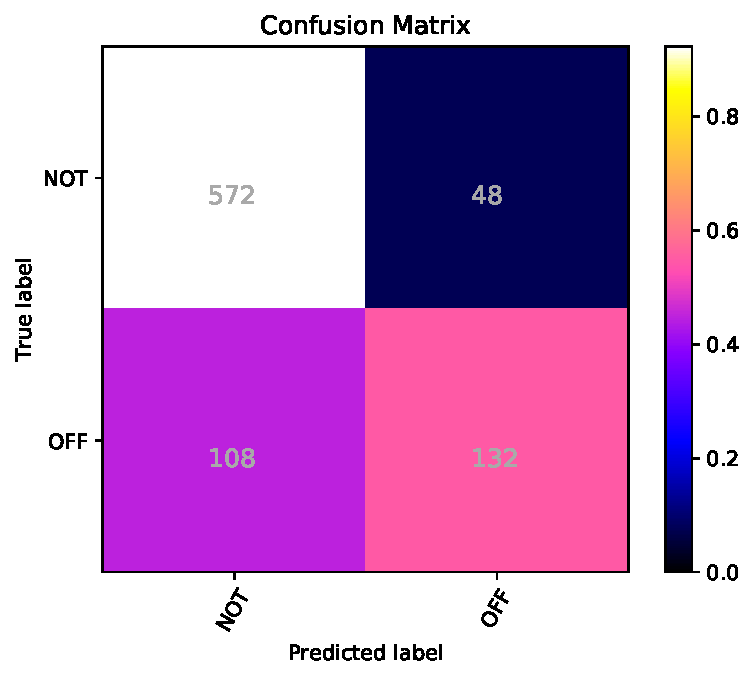
\includegraphics[width=0.5\textwidth]{Sub-task_A,_RyanOng_CodaLab_548951.pdf}
%TODO : add your own details to the caption for this figure
\caption{Sub-task A, RyanOng CodaLab 548951 (WHICH MODEL WAS THIS? ADD YOUR OWN DETAILS HERE)}
\label{fig:1}
\end{figure}


\begin{figure}
\centering
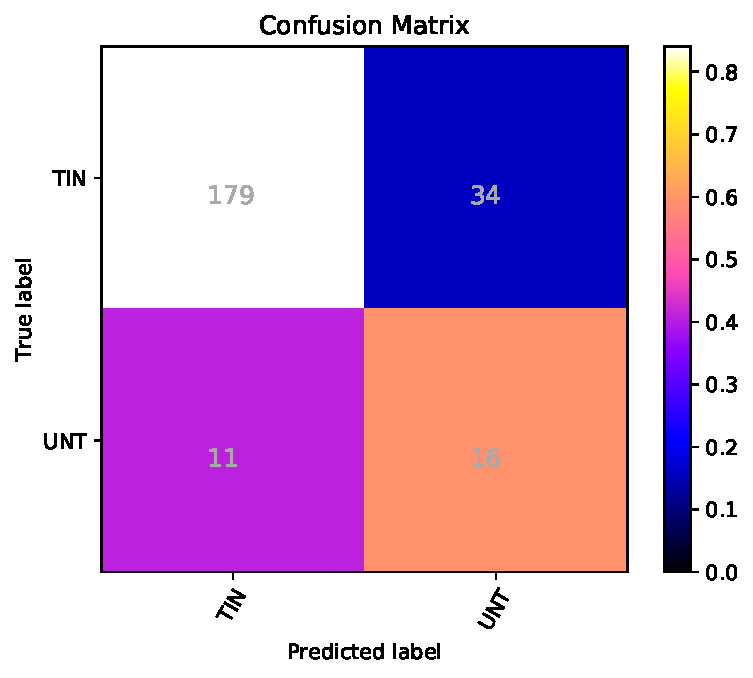
\includegraphics[width=0.5\textwidth]{Sub-task_B,_RyanOng_CodaLab_548986.pdf}
%TODO : add your own details to the caption for this figure
\caption{Sub-task B, RyanOng CodaLab 548986 (WHICH MODEL WAS THIS? ADD YOUR OWN DETAILS HERE)}
\label{fig:2}
\end{figure}


\begin{figure}
\centering
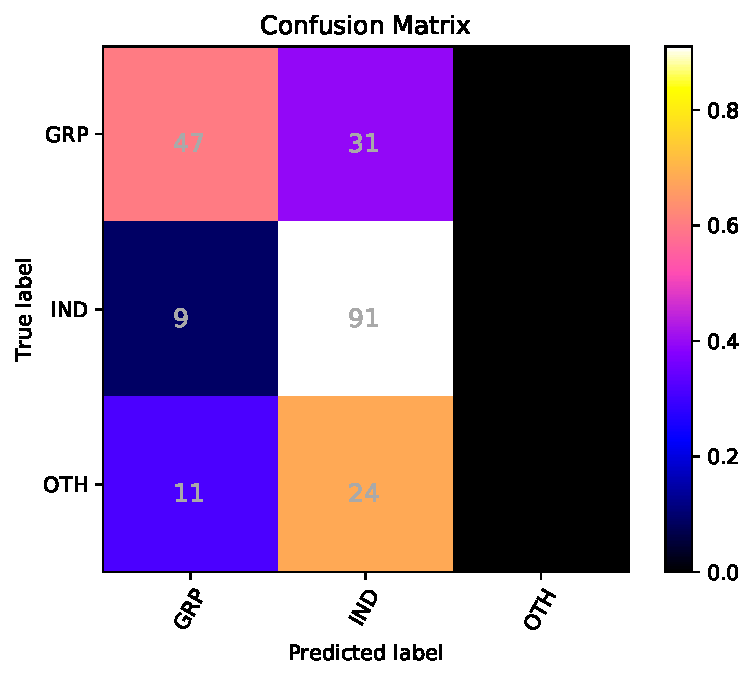
\includegraphics[width=0.5\textwidth]{Sub-task_C,_RyanOng_CodaLab_547628.pdf}
%TODO : add your own details to the caption for this figure
\caption{Sub-task C, RyanOng CodaLab 547628 (WHICH MODEL WAS THIS? ADD YOUR OWN DETAILS HERE)}
\label{fig:3}
\end{figure}


%%%%%%%%%%%%%%%%%%%%%%%%
% REMOVE THIS
% THIS JUST FORMATS THE TEMPLATE WHEN THERE IS LITTLE TEXT
\clearpage % REMOVE THIS LINE
%%%%%%%%%%%%%%%%%%%%%%%%


Feel free to include cross-validation results as well.\\

It is expected that you will interpret and discuss your results here.

\section{Conclusion}

Here you conclude your paper. The readers are interested not only in your system performance but also in what could be learned with your submission.\\

You can also include ideas for future work.

\bibliography{semeval}
\bibliographystyle{acl_natbib}

\end{document}

%%%%%%%%%%%%%%%%%%%%%%%%%%%%%%%%%%%%%%%%%%%%%%%%%%%
% Thank you for participating in OffensEval 2019! %
%                                                 %
% We look forward to reading your system papers.  %
%%%%%%%%%%%%%%%%%%%%%%%%%%%%%%%%%%%%%%%%%%%%%%%%%%%